\subsection{Model Optimizations} \label{subsec:mdopti}
The major issues, when implementing a \acrshort{cnn} on a \acrshort{fpga}, are the \acrshort{cnn} size and its computational complexity. Research has been made to propose techniques to reduce those two elements by directly modifying the \acrshort{cnn} architecture. Moreover, \textcite{nurvitadhi_can_2017} believe that sparsity exploitation and extremely compact data types will become the norm in next-generation \acrshort{cnn}s.
%
%
\subsubsection{Efficient Model Design}
The size of a model can be reduced by changing its architecture. A clever choice of design can reduce the number of parameters and computations. As many approaches have been proposed, we focus our interest on architectures that target the embedded space.

SqueezeNet \cite{iandola_squeezenet_2016} uses an architecture like AlexNet and replaces all layers (except the first and last one) by \textbf{Fire Modules}. The \textbf{Fire Module}, observed in Figure \ref{fig:archi_building_block:sqn}, is a building block where the convolution filter is built of two layers. The first one (squeeze block) is composed only of $1 \times 1$ kernels, which squeeze the number of channels to reduce the computational complexity of the next block. The second one (expand block) is composed of $1 \times 1$ and $3 \times 3$ convolutions. We can reduce, with this architecture, the number of parameters of AlexNet from $240$MB to $4.8$MB. The number of parameters can even be reduced to $0.47$MB with no loss of accuracy from the baseline AlexNet method by applying Deep Compression \cite{han_deep_2016}. However, it has a big memory footprint, is slower in runtime, and consumes more energy than AlexNet \cite{sze_efficient_2017}.

NasNet \cite{zoph_learning_2018} uses a search method, \acrfull{nas}, to find good convolutional architectures on a dataset of interest. NasNet uses a \acrfull{rnn} to generate efficient architectures. The \acrshort{rnn} generates samples child networks with different architecture, which are trained to convergence. The accuracies of the child networks are used to train the \acrshort{rnn}, which will generate better architectures over time. A convolution layer can be seen in Figure \ref{fig:archi_building_block:nasn}. The learned architecture is flexible as it may be scaled in terms of computational cost. However, the resulting network ends up very complex \cite{sandler_mobilenetv2_2019}.

MobileNet \cite{howard_mobilenets_2017} uses \acrshort{dsc}, described in Section \ref{subs:dsc}, to build small and low latency models that can be matched to the design requirements. The layer used is illustrated in Figure \ref{fig:archi_building_block:mbn}. It sets also 2 hyper-parameters to set the model size and throughput: width multiplier $\alpha \in [1; 0[$, which reduces the number of input and output channel at each layer, and resolution multiplier $\rho \in [1; 0[$,  which reduces spatially the input and output \acrshort{fm} at each layer.

ShuffleNet \cite{zhang_shufflenet_2018} is a computation-efficient architecture designed for mobile devices with very limited computing power. It reduces computation cost while maintaining accuracy by using \textbf{pointwise group convolution} which reduces the computation complexity of $1 \times 1$ convolutions. It uses also \textbf{channel shuffle} on the channels such that \textbf{group convolutions} obtain information from different groups. Then more powerful structures can be built with multiple group convolutional layers. However, the group convolutions and the bottleneck structures add \acrshort{mac} which is a non-negligible cost \cite{ma_shufflenet_2018}. The group convolution contributes to network fragmentation and reduces parallelism. Moreover, the \textquote{Add} operation is non-negligible too.

MobileNetV2 \cite{sandler_mobilenetv2_2019} is an improvement of MobileNet in terms of accuracy and does not require special operators. It has also a smaller memory footprint. Furthermore, MobileNetV2 has a faster inference and less parameters with respect to MobileNet. MobileNetV2 has already been explained in Section \ref{subs:mbv2}. The architecture presented by this work has been developed to execute MobileNetV2 because of its simplicity and its state-of-the-art performance (see Table \ref{tab:mbv2}).
%
\begin{figure}
    \centering
    %
    \begin{subfigure}{0.49\linewidth}
        \centering
        \includegraphics[width=\textwidth, height=0.3\textheight, keepaspectratio]{squeeze.pdf}
        \caption{Squeezenet Fire Module\cite{iandola_squeezenet_2016}}
        \label{fig:archi_building_block:sqn}
    \end{subfigure}
    %
    \begin{subfigure}{0.49\linewidth}
        \centering
        \includegraphics[width=\textwidth, height=0.3\textheight, keepaspectratio]{nasnet.pdf}
        \caption{NasNet convolutional blocks \cite{zoph_learning_2018}}
        \label{fig:archi_building_block:nasn}
    \end{subfigure}
    %
    \begin{subfigure}{0.49\linewidth}
        \centering
        \includegraphics[width=\textwidth, height=0.3\textheight, keepaspectratio]{mobilenet.pdf}
        \caption{MobileNet convolutional block \cite{howard_mobilenets_2017}}
        \label{fig:archi_building_block:mbn}
    \end{subfigure}
    %
    \begin{subfigure}{0.49\linewidth}
        \centering
        \includegraphics[width=\textwidth, height=0.3\textheight, keepaspectratio]{shufflenet.pdf}
        \caption{ShuffleNet convolutional block \cite{zhang_shufflenet_2018}}
        \label{fig:archi_building_block:shn}
    \end{subfigure}
    %
    \begin{subfigure}{0.49\linewidth}
        \centering
        \includegraphics[width=\textwidth, height=0.3\textheight, keepaspectratio]{mobilenet2.pdf}
        \caption{MobileNetv2 convolutional blocks \cite{sandler_mobilenetv2_2019}}
        \label{fig:archi_building_block:mb2n}
    \end{subfigure}
    %
    \label{fig:archi_building_block}
\end{figure}

Moreover, a comparison between different architectures is seen in Figure \ref{fig:archi}. We can observe that MobileNetV2 has better accuracy, lower complexity than the previously cited models, and fewer parameters than bigger models.
%
\begin{table}
    \center
    \begin{tabular}{ | c | c | c c | c| }
        \hline \hline
        Network & Top 1 & Params & MAdds & CPU \\
        \hline \hline
        MobileNetV1 & 70.6 & 4.2M & 575M & 113ms \\
        ShuffleNet (1.5) & 71.5 & \textbf{3.4M} & 292M & - \\
        ShuffleNet (x2)  & 73.7 & 5.4M & 524M & - \\
        NasNet-A & 74.0 & 5.3M & 564M & 183ms \\
        \hline
        MobileNetV2 & \textbf{72.0} & \textbf{3.4M} & \textbf{300M} & \textbf{75ms} \\
        MobileNetV2 (1.4) & \textbf{74.7} & 6.9M & 585M & \textbf{143ms} \\
        \hline \hline
    \end{tabular}
    \caption{Performance on ImageNet, comparison for different networks \cite{sandler_mobilenetv2_2019}}
    \label{tab:mbv2}
\end{table}
%
\begin{figure}
    \centering
    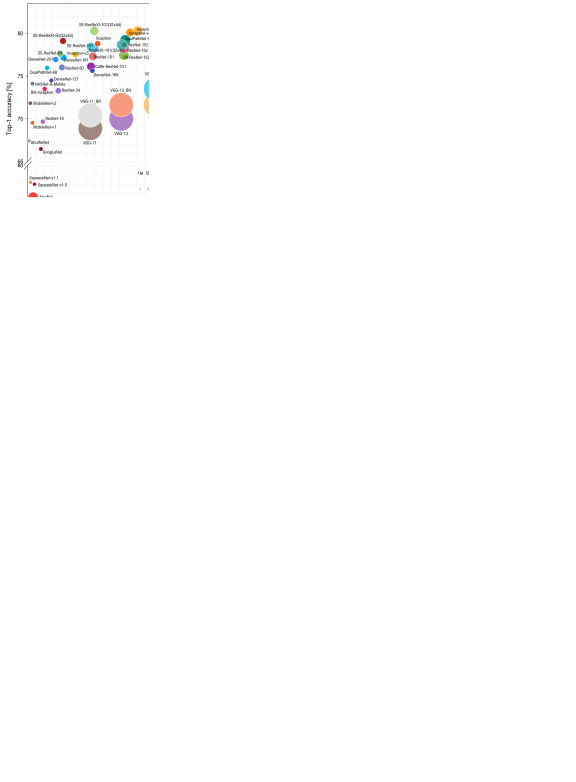
\includegraphics[width=0.9\textwidth]{archi.pdf}
    \caption{Ball chart reporting the Top-1 accuracy of various architectures vs. their computational complexity \cite{canziani_analysis_2017}}
    \label{fig:archi}
\end{figure}
%
\subsubsection{Pruning} \label{subs:pruning}
Network pruning is an effective technique to improve the efficiency of deep networks for applications with limited computational budget \cite{liu_rethinking_2019}. According to \textcite{denton_exploiting_2014, liu_rethinking_2019}, the huge number of parameters in a network creates a problem of \textbf{over-parametrization}. Over-parametrization means that there are redundancies in \acrshort{nn} parameters and we could achieve the same performance with only a subset of them. In consequence, a lot of parameters are unimportant or unnecessary \cite{cheng_recent_2018}. Pruning is defined as removing the parameters considered as not important. For example, \textcite{baoyuan_liu_sparse_2015} achieve more than 90\% sparsity of parameters in convolutional layers in AlexNet with less than 1\% accuracy loss.

We can explain why pruning works by the \textbf{The Lottery Ticket Hypothesis} \cite{frankle_lottery_2019, frankle_early_2020}: \textquote{\textit{A randomly-initialized, dense neural network contains a subnetwork that is initialized such that—when trained in isolation—it can match the test accuracy of the original network after training for at most the same number of iterations.}} From this postulate, we can set to zero (to prune) those unimportant weights because it does not affect the accuracy of the model.

According to \textcite{cheng_recent_2018}, pruning has two major benefits for the inference. First, less storage is required. The non-pruned weights are sparsely distributed among the kernels. Thus, we can store those weights into a compressed format and reduce the memory utilization. Second, we can reduce the arithmetic complexity of the network. As convolutions perform a weighted sum with the input \acrshort{fm}, each \acrfull{mac} operation with a pruned weight can be discarded. Moreover, \textcite{han_learning_2015, mao_exploring_2017, kang_accelerator-aware_2020} pointed that some pruning ratios can also improve the accuracy of the network, which can be explained by a form of regularization.

Various pruning scheme are focused on increasing the sparsity of the network without a drop of accuracy \cite{han_learning_2015, han_deep_2016}.  We call this pruning scheme without constraint \textbf{unstructured pruning}. However, it is challenging to exploit the performance and the high parallelism of \acrshort{fpga} with this kind of pruned network. It is because this kind of pruning scheme creates irregularity in the data access pattern \cite{zhu_efficient_2020}. It means that the number of pruned weights is different in each kernels, and we should adapt the circuitry to the worst case. As a consequence, all filters conduct wasteful operations except the worst case \cite{shimoda_filter-wise_2019}. Furthermore, \textcite{anwar_structured_2017} pointed that unstructured pruning requires an overhead for computing addresses of the sparse non-pruned elements. Therefore, we should find pruning patterns that would be more hardware-friendly.

In contrast to the unstructured pruning, we have \textbf{structured pruning} schemes. It combines a structure regularization for accuracy, and locality optimisation for computation efficiency. Structured pruning has no or little extra costs. We can categorize the various schemes into different groups \cite{wen_learning_2016, anwar_structured_2017, cheng_recent_2018, kang_accelerator-aware_2020}:
\begin{itemize}
    \item \textbf{Depth-wise}: we prune all the weights of a layer. The layer is then removed.
    \item \textbf{Kernel-wise}: instead of pruning all the weights, we keep a ratio of kernels, which mean a reduction of the number of output channel. We can observe the pruning scheme in Figure \ref{fig:struct_pruning:fw}.
    \item \textbf{Channel-wise}: it is one of the most popular method because it still can fit in the convolutional deep learning frameworks \cite{liu_rethinking_2019}. We prune a layer of the input \acrshort{fm}, which means the layer is also pruned in all the kernels. We can observe the pruning scheme in Figure \ref{fig:struct_pruning:chw}.
    \item \textbf{Shape-wise}: we prune the same weight in each kernel, or group of kernels. For example, this pruning scheme has been used in \textcite{zhu_efficient_2020}. It is illustrated in Figure \ref{fig:struct_pruning:sw}
\end{itemize}
%
\begin{figure}
    \centering
    %
    \begin{subfigure}{.32\textwidth}
    \centering
    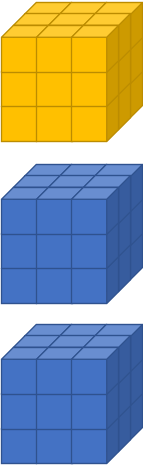
\includegraphics[width=0.33\linewidth]{filterwise.pdf}
    \caption{kernel-wise pruning}
    \label{fig:struct_pruning:fw}
    \end{subfigure}
    %
    \begin{subfigure}{.32\textwidth}
    \centering
    \includegraphics[width=0.33\linewidth]{channelwise.pdf}
    \caption{channel-wise pruning}
    \label{fig:struct_pruning:chw}
    \end{subfigure}
    %
    \begin{subfigure}{.32\textwidth}
    \centering
    \includegraphics[width=0.70\linewidth]{shapewise.pdf}
    \caption{shape-wise pruning}
    \label{fig:struct_pruning:sw}
    \end{subfigure}
    %
    \caption{Structured pruning schemes, where the yellow weights are the pruned ones}
    \label{fig:struct_pruning}
\end{figure}
%
Some works have focused on improving the inference of lightweight models with pruning. \textcite{zhang_channel_2019, tu_pruning_2019} have applied pruning on depthwise separable convolution kernels. They both have chosen \textbf{Channel-wise} pruning because it does not create sparse connection and improves greatly the speed. It also reduces the computational cost of the $1 \times 1$ (pointwise) convolutions, where the majority of the parameters and the \acrshort{mac} comes from. In MobileNet, it is about 95\%. By discarding one channel, we also avoid the associated depthwise convolution.
Moreover, we can prune the pointwise kernel producting that channel in the previous block. We can see the process in Figure \ref{fig:pruning_dsc}.
%
\begin{figure}
    \centering
    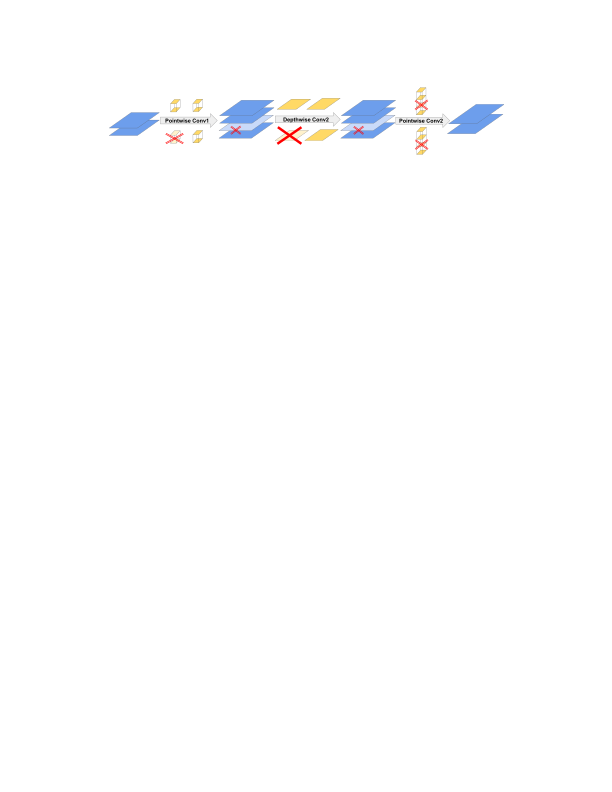
\includegraphics[width=\textwidth]{channelwise_ex.pdf}
    \caption{Pruning a depthwise separable convolution \cite{tu_pruning_2019}}
    \label{fig:pruning_dsc}
\end{figure}

\textbf{In this work we focus on a structured pruning scheme for depthwise separable convolution. More precisely, we develop an architecture on \acrshort{fpga} than combines both advantages of pruning and depthwise separable convolution.}
%
%
\subsubsection{Quantization} \label{subs:quantization}
The approach of quantization is to compress (reducing the bit-width) of floating point parameters to fixed point low-precision parameters. The benefits of quantization, as enonced by \cite{joos_de_ter_beerst_accelerating_2019}, are a reduction of overfitting and an acceleration of computation, since the weights have a smaller bit-size. For example, operations can be four times faster when quantizing to 8 bits due to \acrshort{simd} optimisations.

There are two forms of quantization:
\begin{enumerate}
    \item \textbf{Fixed-point integers}: a number representation using bits is divided into two parts: the first part is dedicated to the integer part and the second one is dedicated to the fractional part of the number. It is easy to implement but it is important to consider the bit size of each part. It can be done by examination after the training. We can also, as for \cite{qiu_going_2016, yin_high_2018}, choose a different range for each layer (doing it for every weight is not memory-efficient).
    \item \textbf{Inteval quantification}: we redefine weights to be between $[-\alpha; \alpha]$. We have to retrain a network before using it but we can achieve good results with a small number of bits. If we fine-tune the network, we can even use 1 (Binary-wheight networks \cite{courbariaux_binarized_2016}) or 2 bits (Ternary-weight networks \cite{li_ternary_2016}).
\end{enumerate}
%
There are also research made on on highly quantized \acrshort{nn} \cite{guo_survey_2018}. Using 16-bits or 8-bits quantization has shown only a small loss in accuracy without retraining \cite{abdelouahab_accelerating_2018}. The quantization of a \acrshort{nn} can be achieved through two different approaches:
\begin{enumerate}
    \item \textbf{Quantification of the weight parameters}: the most widely used. It can be done before or after training, but we have a better accuracy if we quantize during training.
    \item \textbf{Quantification through the activation layer}: we quantize the output of the activation function;
\end{enumerate}
As pointed by \textcite{han_deep_2016}, quantization techniques and pruning are orthogonal and can be combined to compress further the network. Unfortunately, not all existing network are friendly for quantization, like MobileNetV1. Using MobiletNet with quantized pixels and weights, there is a large drop of accuracy (70.50\% usinf floating point model vs 1.80\% using a 8-bit pipeline). However, works of \textcite{sheng_quantization-friendly_2018} have shown that the source of the accuracy drap was the design of the separable convolution core layer. They have therefore proposed a new quantization-friendly separable convolution core layer. Works on MobileNetV2 should then be done to verify the fixed-point inference accuracy. Still, MobileNet had a problem with 8-bit pipeline, increasing the bitwidth to 16-bit could boost accuracy \cite{cheng_recent_2018} and this bitwidth is widely used \cite{huimin_li_high_2016, bai_cnn_2018}. \textbf{Therefore, 16-bit fixed point is adopted for input data, weight and intermediate data}.
